

% \begin{figure}[h]
%     \centering
%     \includegraphics[width=5cm, height=4cm]{Figures/Test_logo.png}
%     \caption{Caption}
%     \label{fig:my_label}
% \end{figure}

\fancyhf{}
\fancyhead[c]{Chapter 4. Timescale Heterogeneity in Reservoir Computing}% <- added
\fancyfoot[R]{\thepage\ifodd\value{page}\else\hfill\fi}
%\fancyhead[L]{\ifodd\value{page}\relax\else\hfill\fi Ch \thechapter}
%\renewcommand\headrulewidth{0pt}% default ist .4pt
\renewcommand{\plainheadrulewidth}{.4pt}% default is 0pt


\newpage


\section{Abstract}

Biological neural systems exhibit significant heterogeneity in the temporal dynamics of their nodes, with neurons operating on a wide range of intrinsic timescales. In contrast, most artificial recurrent networks, including those in the reservoir computing (RC) framework, use homogeneous decay parameters across units. In this work, we investigate whether introducing decay heterogeneity improves task performance in Echo State Networks (ESNs) and Distance-based Delay Networks (DDNs). We evaluate four heterogeneity configurations: homogeneous network, homogeneous cluster, heterogeneous network, and heterogeneous cluster, across two benchmark tasks: NARMA-30 and Mackey-Glass. Networks are optimized using Covariance Matrix Adaptation Evolution Strategy (CMA-ES), and evaluated on task performance, we studied the dynamical stability (Lyapunov exponents), representational dimensionality, and linear memory capacity of these networks. Our results show that DDNs consistently outperform ESNs, with homogeneous DDNs achieving the highest task performance. Timescale heterogeneity enhances memory flexibility in DDNs without compromising stability, while ESNs remain relatively unaffected. These findings suggest that structured heterogeneity in intrinsic timescales significantly improves the computational capabilities of delay-based recurrent systems.

\newpage


\section {Introduction}



Biological networks such as brains consist of nodes with heterogeneous properties; not just in terms of morphology and molecular composition, but also in their temporal properties (\cite{koch1999complexity, habashy2024adapting}). In some cases, differences in timescales among neuron types span several orders of magnitude (\cite{london2010sensitivity, brunel2003firing, wang2020heterogeneity}). This diversity serves multiple functional roles, including supporting motor control (\cite{cavanagh2020diversity}), preserving remote memories (\cite{runyan2017distinct}), and enabling spatial memory formation (\cite{mcnaughton2006path}). In particular, variation in neuronal time constants and decay dynamics is thought to be critical for temporal processing and memory formation in the brain (\cite{hasson2008hierarchical, chu2020long}).

In contrast, artificial neural networks, especially recurrent neural networks and their variants like the reservoir computing (RC) framework, are typically designed with homogeneous units that share identical intrinsic parameters. RC is a powerful approach for modeling temporal sequences (\cite{lukovsevivcius2009reservoir}), a well known RC system is an Echo State Networks (ESNs) (\cite{jaeger2001echo}). Originally, these networks rely on a fixed, randomly connected recurrent reservoir, whose states are linearly read-out by a trainable readout layer. This setup simplifies training while maintaining a strong performance on memory-intensive and nonlinear tasks, particularly time dependent and sequential tasks. A key hyperparameter in RC systems is the leak or decay rate of the reservoir neurons, which controls how much past information is taken into account in each unit, shaping the network's temporal memory (\cite{schrauwen2007overview}).

Recently, an extension of ESNs called Distance-based Delay Networks (DDNs) (\cite{iacob2022distance}) has been introduced. DDNs incorporate non-uniform delays between reservoir units, motivated by the fact that axonal delays are ubiquitous in the brain and that information in physical systems like the brain is constrained by the spatial structure and finite signal transmission speed (\cite{izhikevich2006polychronization}). Prior work has shown that these heterogeneous delays lead to a redistribution of memory across timescales and can improve task performance compared to standard ESNs (\cite{iacob2022distance, soriano2014delay, perez2021neural}).

The role of inter-unit delays has been much explored, it remains unclear whether heterogeneity in intrinsic parameters - specifically decay rates can further enhance performance in both ESNs and DDNs. Most prior studies assume a single, homogeneous decay parameter across all units, effectively enforcing a single timescale on the reservoir. This may limit the system's ability to capture rich, multi-timescale dynamics, especially in tasks that demand both short- and long-term memory. In contrast, biological neural systems inherently operate with a range of time constants (\cite{london2010sensitivity, nam2017diversity, zhou2023temporal}), suggesting that incorporating decay heterogeneity could yield computational benefits.

To investigate the effect of intrinsic timescale heterogeneity on network performance, we design and analyze two sets of reservoir networks, ESNs and DDNs, each implemented in four different configurations. These include 1.) a homogeneous setup where all units share a fixed decay value, 2.) a fixed-cluster configuration, where the reservoir is divided into modules, each with its own fixed decay, 3.) a network-heterogeneous configuration, where each unit's decay is sampled independently from a common distribution; and 4.) a cluster-heterogeneous configuration, where different modules sample their decays from different distributions. We evaluate all configurations on two standard benchmark tasks: the NARMA-30 task, which tests nonlinear memory capacity, and the Mackey-Glass task, which involves chaotic time-series prediction. Performance is optimized using a Covariance Matrix Adaptation Evolution Strategy (CMA-ES), with task evaluation based on the normalized root mean square error (NRMSE) for NARMA and the prediction horizon for Mackey-Glass.

Beyond performance, we analyze the networks' internal dynamics to understand the mechanisms underlying any observed differences. We compute Lyapunov exponents to assess dynamical stability and chaotic behavior, measure representational dimensionality using SVD-based metrics, and evaluate linear memory capacity. Our results show that DDNs consistently outperform ESNs across all heterogeneity types, with fixed-cluster DDNs performing best. These findings suggest that structured temporal heterogeneity, particularly when organized in modular clusters, significantly enhances the computational capabilities of reservoir networks for tasks involving memory and temporal dynamics. 

 

\newpage


\section{Methods}



\subsection{Network Design}

\subsubsection{Echo State networks }

Echo state networks (ESN) (\cite{jaeger2001echo}) are essentially recurrent networks with fixed weights and randomly connected units given by the following equation: 

\begin{equation}
    X(n+1) = (1-\alpha)X(n) + \alpha f(W_{res}X(n) + b_{res} + W_{in}V(n)) ,
\end{equation}
 
Where $X(n)$ represents the state of the reservoir at time step $n$. The size of the reservoir is given by the number of units $N$. The symbol $W_{res}$ is the $N \times N$ weight matrix of the reservoir. Symbol $W_{in}$ represents a $N_{in} \times N$ input weight matrix, where $N_{in}$ in the number of input nodes. $b_{res}$ represents the bias of the reservoir nodes, $V(n)$ is the input to the reservoir at time step $n$, $\alpha$ is the leak parameter, which decides the importance of previous states on the current state, therefore acting as a memory decay parameter. Contrary to RNNs, only the linear readout layer is trained for an ESN in order to optimize it for a task. This leak parameter can be fixed or variable for each unit. $f(\cdot)$ is the non-linear activation function, which is usually sigmoid or hyperbolic tangent.     

\subsubsection{Distance based delay networks}

The architecture of Distance based Delay networks (\cite{iacob2022distance}) are similar to ESNs except for the introduction of delays. The delays are implemented by assuming that each unit lies on a 2-D Euclidean plane and the distance between two units determines the delay between them. A distance matrix $D$ is computed, where each element $D_{ij}$ represents the distance between units $i$ and $j$ scaled by the signal propagation velocity and simulation timestep. A new masked weight matrix $W^{res}_{D=d}$ is created accounting for delays, each element in this matrix is given by the following equation:

\begin{equation}
    W_{i,j,D=d} = \delta_{i,D_{ij}} \cdot W_{i,j}, 
\end{equation}

where, d $\in$ [$1$, $D_{max}$] and $\delta$ is the Kronecker delta operator.  $D_{max}$ is the maximum value delay can take. The final update equation for DDNs is given by: 
\begin{equation}
i(n)  = \sum_{d=0}^{D_{max}} \bigg( W^{res}_{D=d} x(n-d) + W^{in}_{D=d} v(n-d) \bigg ) + b_{res} \\
\end{equation}
\begin{equation}
    x(n) = (1-\alpha) x(n-1) + \alpha f(i(n)) 
\end{equation}

All the parameters in the above set of equations are identical except for the addition of delays. As described in \cite{iacob2022distance}, the delay between individual units are treated as hyperparameters to be optimized. During initialization, the coordinates of the neurons are sampled using a Gaussian Mixture model, with $K$ number of clusters. Instead of finding the optimal coordinates for each unit, the GMM model is optimized to find the fitting distribution for each cluster.  

\subsection{Task}

\subsubsection{NARMA-30}
The Nonlinear Auto-Regressive Moving Average (NARMA) is a popular benchmark task used to evaluate the performance of an RC system. It is a system that is highly non-linear and has clear temporal dependencies such that the current state depends on the past states, defined by the order parameter $p$, which decides the time step up until which the dependency is carried out. The general equation is given by: 

\begin{equation}
    y(t+1)  = c_1 \cdot y(t)+c_2 \cdot \sum_{i=0}^{p} y(t-i) + c_3 \cdot u(t-p)u(t) +c_4, 
\end{equation}
where $c_1$ -- $c_4$ are task parameters, and $p$ is the NARMA order. $y(t)$ is the state of the system at time t, $u(t)$ is the input to the system at time $t$, which is uniformly sampled between $0.0$ and $0.5$. Essentially, the NARMA task entails predicting the next state of the system $y(t+1)$ given the serialized previous states of the same system. In this study we used the NARMA-30 task to train our networks, the parameters for the task are following,  $p = 29$, $c_1 = 0.2$, $c_2 = 0.004$, $c_3 = 1.5$, and $c_4 = 0.1$. 

\subsubsection{Evaluation}
We evaluated the NARMA-30 task using the Normalized Root Mean Squared Error (NRMSE) given as follow: 
\begin{equation}
    NRMSE = \frac{1}{\bar{y}}\sqrt{\frac{\sum (y_i - \hat{y}_i)^2}{n}}      
\end{equation}
where $\bar{y}$ is the mean of the ground truth, $y_i$ and $\hat{y}_i$ are ground truth and network readout respectively, and $n$ is the total number of elements in the time series.     

\subsubsection{Mackey-Glass}

The discretized Mackey-Glass timeseries is given by the following equation:

\begin{equation}
    x(t+1) = x(t) + \beta\frac{x(t-\tau)}{1+x(t-\tau)^{n}} -\gamma x(t)
\end{equation}
The parameters were chosen as follows, $\tau = 17$, $n = 10$, $\beta = 0.2$ and $\gamma = 0.1$. The aim of the Mackey-Glass is to accurately generate the Mackey-Glass sequence as long as possible using the previous step and not receiving any external input or correction. This is done by training the readout layers of the networks for one step ahead prediction, this involves comparing the network prediction based on the previous step as input. The performance is measured by a metric called prediction horizon, which measures how many time steps into the future can be predicted by the network accurately within an error margin.

\subsubsection{Evaluation}
We evaluated the network performance using the prediction horizon, which the number of time steps the network can predict the time series within the error margins. The error margins are $\pm 0.1\sigma^{2}_l$, where $\sigma^{2}_l$ is the label variance. 

\subsection{Training}
\subsubsection{CMA-ES Optimization}
The Covariance Matrix Adaptation Evolution Strategy (CMA-ES) (\cite{hansen2006the-cma-evoluti}) is a widely used evolutionary algorithm for hyperparameter optimization, especially effective for non-convex and high-dimensional problems. CMA-ES consists of a multivariate Gaussian search distribution defined by a mean vector, step-size, and covariance matrix. At each iteration, it samples a population of candidate solutions from this distribution, evaluates their fitness, and updates the mean and covariance matrix to sample future samples from more fitting regions of the search space. The mean vector represents the current best candidate based on the population's progress, while the covariance matrix spans the space of the search distribution. This iterative process enables CMA-ES to efficiently explore complex solution spaces and is robust to non-convexity, noise, and ill-conditioned search landscapes, due to its invariance properties and ability to handle parallel evaluations. In case of ESN and DDN optimization, the mean vectors are the hyperparameters of DDNs and ESNs. Initially, all hyperparameters are roughly made to fall in the same range, after every iteration, a new hyperparameter vector is generated based on the evolution of the multi-variate distribution. Using this new solution vector, networks are generated and are used to perform validation scores. Both ESN and DDN optimizations are run for 200 generations with a population size of 20 for Mackey Glass task and population size 25 for NARMA 30 task. 


\begin{table}
    \centering
    \begin{tabular}{p{3cm}|p{1.5cm}|p{5cm}|p{3cm}}
         Parameter&  Symbol &  Description& Size\\
        \hline
        \hline
         Mixture Components&  $\phi$&  Distribution of neurons among sub-reservoir. & $K$\\ 
         
         Cluster Mean&  $\mu$&  Spatial mean of neuron clusters& $K \times D_s$\\
         Cluster Covariance & $\Sigma$ & The covariance matrix of neuron locations. & $K \times D_s \times D_s$ \\
         
         Weight Scaling & $S_{res}$  & Scaling factor for inter and intra-reservoir weights. & $(K+1) \times (K+1)$  \\
         
         Bias Scaling & $S_b$ & Scaling factor for bias weights for each sub-reservoir.  & $K$ \\ 
         
         Connectivity& $C$  & Inter- and intra-cluster connectivity, expressed as a fraction of full connectivity, structured in a matrix. & $(K+1) \times (K+1)$\\
         Leak rate & $\alpha$ & The leak rate as shown in eq. (1) and (4).  & K or mean and variance of each cluster or for the entire network. \\
         \hline
         \hline
    \end{tabular}
    \caption{Summary of the hyperparameters optimized by the CMA-ES algorithm for ESNs and DDNs, expressed as the number of clusters $K$ and spatial dimensions $D_s$.}
    \label{tab:placeholder}
\end{table}
\subsubsection{Readout training}
The randomly sampled network is not directly able to perform the task, it is essentially it acts as a temporal kernel that increases the dimensionality of the input and thus increases the linear separability. The activity from a network driven by a random input can be recorded and can be treated as a feature matrix $X$ of size $N\times T$, where $N$ is the number of neurons and $T$ is the number of time steps of the simulation. The output labels $\hat{y}$ and and the corresponding input vector $v(n)$ are ordered vectors of size $T$. The objective function $J$ given by the following equation below is solved using ridge regression trained on network activities: 
\begin{equation}
    J(W_{readout}) = ||XW_{readout}  - \hat{y} ||_2 + \lambda || W_{readout}||_2,
\end{equation}
Optimizing the above equation gives the $W_{readout}$, where $\lambda$ is the regularizing parameter and $W_{readout}$ is the readout weight. The $W_{readout}$ matrix is randomly sampled during initialization.  

\subsection{Lyapunov exponent}

The dynamics of the RC system can be studied by estimating the Lyapunov exponent of the network trajectory. We calculated the Lyapunov exponent of ESNs and DDNs using a numerical method, explained by \cite{boedecker2012information}. The Lyapunov exponent is given by the following equation: 
\begin{equation}
    \lambda = \lim_{t \to +\infty} \frac{1}{t} ln \bigg ( \frac{\gamma_t}{\gamma_{0}} \bigg ),
    \label{eq:lyapuno}
\end{equation}
where $\lambda$ is the Lyapunov exponent, $\gamma_t$ and $\gamma_0$ are distance between normalized distance between entities at time t and during initialization, respectively.  
The steps involved in the numerical calculation as described by \cite{boedecker2012information} is as follows:
\begin{enumerate}
    \item Two identical networks $X_1$ and $X_2$ were created taking the best sampled networks from the CMA-ES optimization. A reservoir unit from one of the network $X_1$ was given a small perturbation and the network $X_2$ was kept as is. The initial $L2$ normalized distance between $X_1$ and $X_2$ is therefore $\gamma_0$.   
    \item The network is driven by the input that the network is trained on, that is either NARMA-30 or Mackey-Glass inputs. At each simulation step $t$ a normalized $L2$ distance between networks $\gamma_t = ||X1(t)-X2(t)||_2$ is calculated. 
    \item   The perturbed network $X_1$ is reset to the initial distance $\gamma_0$, $X_1 \to X_2(t)+(\gamma_0/\gamma_t)(X_2(t) - X_1(t))$   once it crosses the upper or lower thresholds, i.e, $\gamma_t \notin [1e^{-5}, 1e^{-14}]$, this step is essential to prevent numerical overflows.
    \item     The simulation is run and averaged over for 200 steps, and is repeated and saved for multiple perturbation intensities ranging from $1e^{-1}$ to $1e^{-9}$ for comparison. Finally the Lyapunov exponent is given by the equation \ref{eq:lyapuno}.    
\end{enumerate}

The above steps are repeated for all the networks for both the tasks. All the numerical simulations were performed using python and TensorFlow 1. 

\subsection{Dimensionality}

The dimensionality of a given network while performing a task was calculated using Singular Vector decomposition \cite{jordanou2023investigation} of the activity matrix and counting the top singular values that explain 99\% of the variance, this threshold is denoted with $EV_{\theta}$. The SVD is given as follows:
\begin{equation}
    A = U \Sigma V^T
\end{equation}
where $U$  of and $V^T$ are left and right singular matrices of dimensions $N\times N$ and $T \times T$ respectively, $\Sigma$ is the diagonal matrix of dimensions $N \times T$. The dimensionality is given by:
\begin{equation}
dim = \frac{\sum_{i=1}^{n}\sigma_{i,i}}{\sum_{i=1}^{N}\sigma_{i,i}} >= EV_{\theta} ; n < N   
\end{equation}
where $\sigma_{i,i}$ are the diagonal elements of the singular value matrix $\Sigma $, N is the number of reservoir units in ESNs and DDNs and $n$ is the number of units that are enough to reach the $EV_{\theta}$ threshold.  

\subsection{Linear Memory Capacity}

Linear Memory Capacity measures short term memory distribution of a dynamical system (\cite{jaeger2001short}).  In order to calculate the linear memory capacity, the ENSs and DDNs are driven with a uniform random input and the readout layer is trained to reproduce the input from time lag ($l$) ago. The linear memory capacity at a specific lag $l$ shows how well the reproduction by a network correlates with the input $l$ time steps ago.  The total memory capacity is given by summing all the memory capacities for each lag. The idea is formulated as follows: 
\begin{equation}
    MC_l = r(u(n-l), \hat{u}(n))^2
\end{equation}
\begin{equation}
    MC_{total} = \sum_{l=1}^{\infty} MC_l
\end{equation}
Where $r(\cdot)$ is the Pearson correlation, $u(n)$ is the input at timestep $n$ and $\hat{u}(n)$ is the readout reproduction of the input at timestep $n-l$. It is important to note that the networks for the MC calculations are taken after the parameters are optimized using CMA-ES method and their linear readout is trained for a specified task.   


\newpage

\section{Results}

The aim of this study was to study the effect of intrinsic heterogeneity on task performance of ESNs and DDNs. Therefore we designed 4 heterogeneity/homogeneity configurations as follows: 

\begin{enumerate}
    \item \textbf{Homogeneous Network}: All units share a single decay parameter.
    \item \textbf{Homogeneous Cluster}: The reservoir is divided into clusters, each with its own fixed decay parameter.
    \item \textbf{Heterogeneous Network}: Each unit samples its decay from a shared distribution.
    \item \textbf{Heterogeneous Cluster}: Each cluster samples decay parameters from different distributions.
\end{enumerate}
The size of the cluster in case of both homogeneous and heterogeneous clusters is chosen to be 4, during the CMA-ES optimization, the actual size of the cluster might change, as it is also hyperparameter to be optimized. 

These configurations are tested on two benchmark tasks namely NARMA-30 and Mackey-Glass tasks (see Methods section 5.2):
\begin{itemize}
    \item \textbf{NARMA-30}: A nonlinear auto-regressive moving average task designed to test long-range memory and nonlinear dynamics. Parameters for the NARMA-30 task are given in Methods section 5.2.1. 
    \item \textbf{Mackey-Glass}: A chaotic time-series prediction task that evaluates a network's ability to generate stable yet complex temporal outputs. Parameters for the Mackey-Glass task are given in Methods section 5.2.2. 
\end{itemize}

A key reason to optimize network for these two tasks is to understand if inherent heterogeneity is utilized based on task performance. We optimized all network hyperparameters using the CMA-ES learning algorithm (see Method section 5.3). We evaluated the task performance for NARMA-30 and Mackey-Glass tasks using NRMSE and prediction horizon measures respectively (see Method section 5.1).  

\begin{figure}
    \centering
    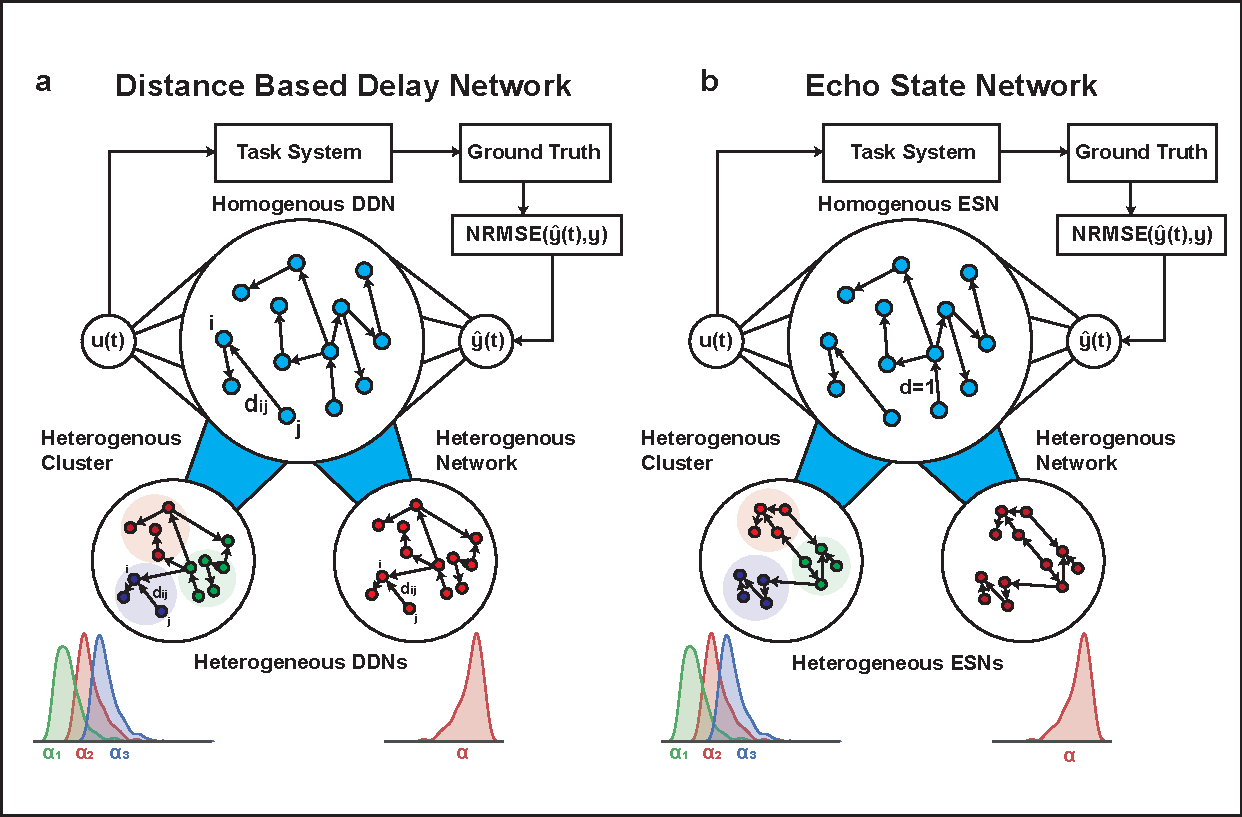
\includegraphics[width=\linewidth]{Figures/Ch_4/network_architecture.pdf}
    \caption{\textbf{Reservoir architecture and heterogeneity design in DDNs and ESNs:} \textbf{(a)} DDNs were made heterogeneous by introducing heterogeniety in decay ($\alpha$), cluster heterogeneity is designed by sampling decays from different distributions for each cluster, similarly, network heterogeneity is designed by sampling decays from a single distribution. \textbf{(b)} same heterogeneity designed for ESNs.    }
    \label{fig:reservoir-arch}
\end{figure}



\subsection{Task Performance }
\subsubsection{NARMA 30}

In order to study the effect of heterogeneity in leak parameters in ESNs and DDNs, we evaluated the networks using their validation scores for each generation (see Methods) of CMA-ES algorithm while these networks learn to perform NARMA-30 task (see Methods). In \textbf{Fig. \ref{fig:eval}a} it can be seen that as the networks are optimized over generations, the validation scores decrease for both ESNs and DDNs, but the NRMSE scores for DDNs, especially DDNs with a homogeneous network parameter, a heterogeneous cluster and a homogeneous cluster architecture, are much lower than ESNs. It can also be seen that all ESNs eventually lead to similar NRMSE scores. Interestingly, DDNs with homogeneous cluster out perform DDNs with higher levels of heterogeneity, and the DDNs with heterogeneous network architecture show a similar performance to the ESNs. 

We evaluated the performance of the best optimized networks on a test set within ESN and DDN heterogeneity architectures and between ESN and DDN architectures. In \textbf{Fig. \ref{fig:eval}b}, it can be seen that DDNs with homogeneous network architecture has significantly lower NRMSE score than ESNs with homogeneous network architecture (t(28) = -19.79129, p = 5.3404 e-18), same with DDNs with heterogeneous network architecture (t(28) = -19.79129, p = 5.34047e-18). With similar comparison for cluster heterogeneity between DDNs and ESNs, we found that DDNs with homogeneous cluster have significantly lower NRMSE scores than ESNs (t(28) = -6.18253, p=1.1214e-06) and for heterogeneous cluster architecture, we also found that DDNs have significantly lower NRMSE scores than ESNS (t(28) = -5.68152, p = 4.3262e-06).     

We also compared the test scores between architectures for ESNs and DDNs for both heterogeneous network and heterogeneous cluster case. We find that DDNs with heterogeneous network architecture perform significantly worse than DDNs with homogeneous network architecture (t(28) = 20.38542, p = 2.4574e-18) and we observe the same for ESNs (t(28) = 3.72274, p = 8.7914e-4). We compared the cluster heterogeneity and found that difference between NRMSE score for DDNs with homogeneous cluster and heterogeneous cluster was not significant. While ESNs with homogeneous cluster showed significantly lowered NRMSE score than heterogeneous cluster counterparts (t(28) = 4.4671, p = 1.1882e-4).  

These results indicate that although ESNs converge to similar NRMSE scores across generations, DDNs show performance differences based on the organization of leak parameter heterogeneity. Specifically, DDNs with per-cluster fixed decay achieve significantly lower validation and test errors compared to ESNs and other DDN configurations, highlighting the advantage of structured heterogeneity. Higher levels of heterogeneity, such as network-wide distributed decay, result in DDN performance comparable to ESNs, suggesting that unrestricted variability can diminish the benefits. Overall, constrained per-cluster heterogeneity in leak parameters appears to optimize network performance on the NARMA-30 task.

\subsubsection{Mackey-Glass}

To understand whether the optimal level of heterogeneity depends on the task the network is trained to perform, we trained ESNs and DDNs with four types of heterogeneity configurations on a different kind of task. Similar to the NARMA-30 task, we optimized ESNs and DDNs with varying levels of heterogeneity for the Mackey-Glass time series prediction task (see Methods section). We evaluated the performance of the networks using the prediction horizon metric (see Methods section). In Fig. \ref{fig:eval}b, we show that prediction horizons during validation across generations of CMA-ES optimization for DDNs are consistently higher than for ESNs. It can also be seen that DDNs with a network-wide distributed decay perform the best among all DDN variants, reaching a prediction horizon of 500 steps. Notably, ESNs with per-cluster distributed decay and network-wide fixed decay perform the worst compared to all other variants. ESNs with network-wide distributed decay and per-cluster fixed decay perform objectively better, reaching a prediction horizon of 300 steps. 


Similar to the NARMA-30 task, we evaluated the performance of the best optimized networks on a test set within ESN and DDN heterogeneity architectures and between ESN and DDN architectures. In \textbf{Fig. \ref{fig:eval}d}, it can be seen that DDNs with homogeneous network architecture has significantly higher prediction horizon score than ESNs with homogeneous network architecture (t(8) = 4.77824, p = 1.3938e-3),  while DDNs with heterogeneous network architecture show significantly worse performance than ESNs with heterogeneous network architecture (t(8)=-3.98428, p = 4.0374e-3). With similar comparison for cluster heterogeneity between DDNs and ESNs, we found that DDNs with homogeneous cluster have significantly higher prediction horizon scores than ESNs (t(8) = 10.01157, p = 8.4151e-06) and for heterogeneous cluster architecture, we also found that DDNs have significantly higher prediction horizon scores than ESNS (t(8) = 8.33998, p = 3.2324e-05).     


We also compared the test scores between architectures for ESNs and DDNs for both heterogeneous network and heterogeneous cluster case. We find that DDNs with heterogeneous network architecture perform significantly worse than DDNs with homogeneous network architecture (t(8) = 4.20005, p = 2.9962e-3) and we the opposite for ESNs, ESNs with heterogeneous network perform better than ESNs with homogeneous network (t(8) = -4.2618, p = 2.7543e-3). We also compared the cluster heterogeneity and found that difference between prediction horizon score for DDNs with homogeneous cluster and heterogeneous cluster was significant (t(8) = -13.19701, p = 1.0355e-06). ESNs with heterogeneous cluster showed significantly higher prediction horizon score than homogeneous cluster counterparts (t(8) = -5.92572, p = 3.5142e-4).  


Together, these findings suggest that the effect of heterogeneity on network performance is strongly influenced by both the underlying architecture and the specific task, with DDNs showing overall superior predictive capability and heterogeneous cluster architecture configurations providing the most consistent improvement. This suggest that heterogeneity improves the performance for DDNs and ESNs but the level of heterogeneity required is task dependent. 


\begin{figure}
    \centering
    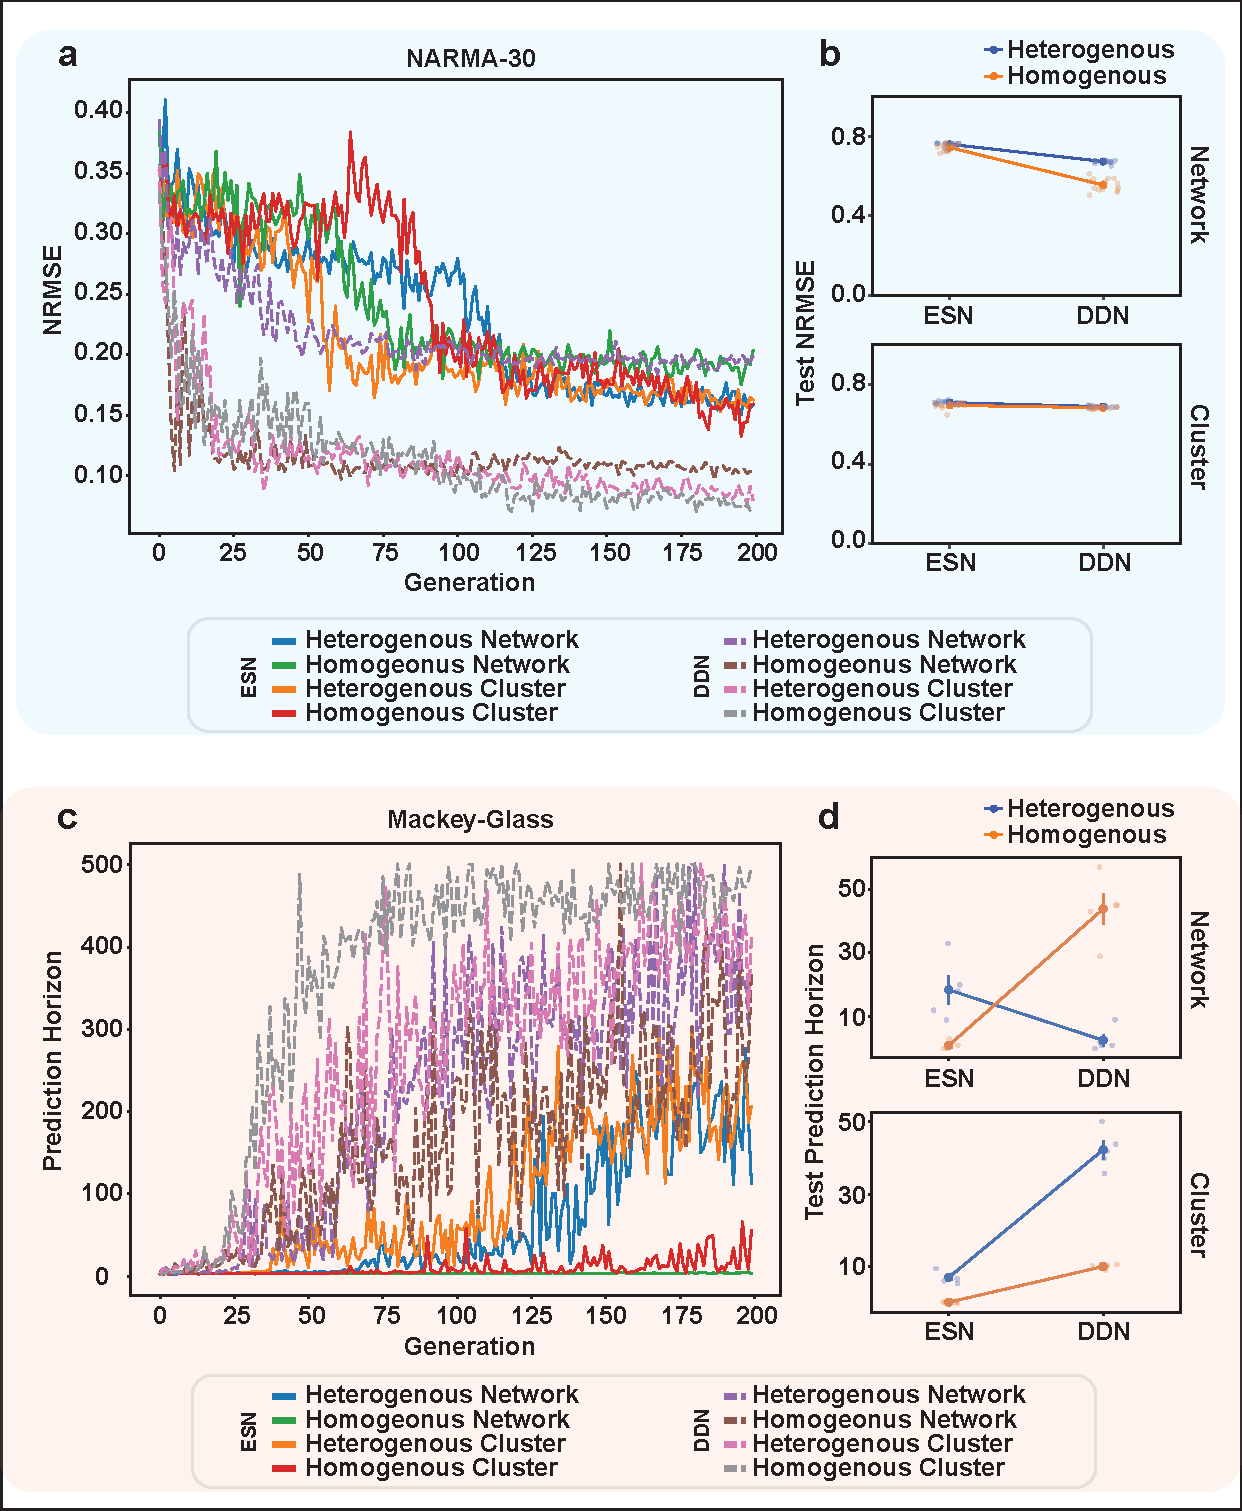
\includegraphics[width=\linewidth]{Figures/Ch_4/Task_performance.pdf}
    \caption{\textbf{Network performance for DDNs and ESNs with or without heterogeneity}: \textbf{(a)} Line plot shows the perforamce in terms of NRMSE over generation during CMA-ES optimization for DDNs and ESNs during NARMA 30 task.}
    \label{fig:eval}
\end{figure}

\begin{figure}

\textbf{(b)} Test NRMSE for the optimized network for both ESNs and DDNs in different heterogeneity configurations. It can be seen that DDNs with/without heterogeneity perform better than ESNs. \textbf{(c)} Performance of ESNs and DDNs with or without heterogeneity optimized for Mackey-Glass prediction task over generations of CMA-ES optimization. \textbf{(d)} Test performance of ESNs and DDNs optimized for Mackey-Glass timeseries prediction task, separated based on heterogeneity types. * $p<0.05$, ** $p<0.001$, *** $p<0.0001$.
\end{figure}

\subsection{Stability and Dimensionality}
\subsubsection{Maximum Lyapunov Exponents}
In order to evaluate the advantage of intrinsic heterogeneity on ESNs and DDNs we calculated the maximum Lyapunov exponents (MLE) of the sampled best networks while they perform the task (see Methods section). This was done in order to examine the stability of the network dynamics while the networks perform the task. We hypothesized that intrinsic decay heterogeneity might cause the networks to be more chaotic than their homogeneous counterparts. We evaluated the Maximum Lyapunov exponents for each network and heterogeneity type for different perturbation magnitudes ranging from $1e^{-1}$ to $1e^{-9}$. We perform this analysis for NARMA-30 and Mackey-Glass tasks separately, the results are summarized in \textbf{Fig. \ref{fig:lyapunov}a-b}. 

For NARMA-30 task (\textbf{Fig. \ref{fig:lyapunov}a}), it can be seen that for each perturbation magnitude, the largest Lyapunov exponents are negative for all ESNs variants and are lower than those of DDNs, suggesting that ESNs have more contracting dynamic than DDNs despite the decay heterogeneity in the network architecture, as can be seen for example in ESNs with heterogeneous cluster (purple solid line) and DDNs with heterogeneous cluster (dark brown dotted line). The outlier to this observation is the ESN with network wide fixed delay (lemon green solid), for which the Lyapunov exponent is negative but invariant to the perturbation magnitude and comparable to DDNs. It is also important to observe that for all perturbation magnitudes, the highest perturbation yields the lowest exponent. In case of DDNs, the per cluster fixed decay configuration the maximum Lyapunov exponent was invariant to the perturbation magnitude. The MLE for DNNs with network wide distributed decay (dotted cyan) and per cluster distributed decay (dotted brown) were comparable. On the other hand, DDNs with network wide fixed decay shows a positive MLE for highest magnitude perturbation ($1e^{-1}$) suggesting chaotic dynamics. We compared the MLE for each optimized network with their respective best validation performance (Fig. \ref{fig:lyapunov_vs_perf} \textbf{a}), it can be seen that in case of NARMA-30 task, the best performing DDNs (low NRMSE)  have a higher MLE than best performing ESNs. The overall best performing network, DDN with homogeneous cluster, doesn't have higher MLE than other DDNs. Suggesting that even though DDNs have less contracting dynamics than ESNs, the best performance doesn't linearly depend on the MLE of the network.  

For the Mackey-Glass timeseries prediction task (\textbf{Fig. \ref{fig:lyapunov}b}), it can be seen that for each perturbation magnitude, the maximum Lyapunov exponent is negative for all ESNs variants and these are lower than that of DDNs, suggesting that ESNs have more contracting dynamic than DDNs for this task as well. It is also important to observe that for all perturbation magnitudes, the highest perturbation yields the lowest exponent just as in case of NARMA-30. The ESNs with network wide distributed decay were found to have the highest MLE among ESNs and the ESNs with per cluster fixed decay were found to have the lowest MLE. In case of DDNs, the per cluster fixed decay configuration shows a positive exponent for the  magnitude of $1e^-9$ and $1e^-7$. The MLE for DNNs with all other variants had comparable negative MLE for all each perturbation magnitude suggesting a stable contracting dynamic. We compared the network performance and MLE for each network for the Mackey-Glas task (\textbf{Fig.} \ref{fig:lyapunov_vs_perf} \textbf{b}). It can be seen that even though all DDNs learn to perform the task as seen from the max prediction horizon, the DDNs with most contracting dynamics are the DDNs with heterogeneous and homogeneous clusters. It can also be seen that ESNs with network heterogeneity and cluster heterogeneity, that performs relatively better than other ESNs, have lower MLE than their counter parts. The figure also suggests that, even thought ESNs have lower MLE, it doesn't correlate with their performance. DDNs with higher MLE perform the task better.   

Overall, the Lyapunov exponent analysis indicates that decay heterogeneity does not inherently destabilize reservoir dynamics but instead yields nuanced, task- and architecture-specific effects. For both NARMA-30 and Mackey-Glass tasks, ESNs consistently exhibited strongly contracting dynamics relative to DDNs, underscoring their robustness across perturbation magnitudes, even under heterogeneous configurations. While certain DDN variants demonstrated positive exponents at specific perturbation scales, suggestive of localized chaotic regimes, the majority of configurations maintained negative exponents, consistent with stable information processing. These results suggest that intrinsic heterogeneity can be integrated into recurrent architectures without compromising dynamical stability, and may underlie functional benefits that are task dependent.

 
\subsubsection{Dimensionality}
In order to further evaluate the usefulness of intrinsic heterogeneity in terms of recruiting reservoir units for performing a task, we calculated the dimensionality of the network activity using the network states during network simulations driven by the task input. We hypothesized that intrinsic decay heterogeneity might increase the dimensionality of the network, improving the task performance. We drove the network with NARMA-30 and Mackey-Glass input for 2000 steps, and used the network states after a 300 step of warm-up period. For NARMA-30 task, we observed a low dimensionality for all networks. 


The highest dimensionality was obtained for DDN with homogeneous cluster (D=18) and the lowest for DDNs with a heterogeneous cluster (D=7). ESNs on the other hand show high dimensionality (D=14) for heterogeneous cluster (purple) and homogeneous network (olive) configuration.  Comparing the performance of networks as a function of dimensionality for NARMA-30 task (\textbf{Fig. \ref{fig:lyapunov_vs_perf} c}), we see that network that performs the best, DDN with homogeneous cluster has higher dimensionality than other networks. It is also important to observe that DDN with heterogeneous cluster (pink) although has comparable performance, has lower dimensionality. This suggests that heterogeneity affects dimensionality of the network but improvement in performance is not linearly dependent. 

Similarly, for the Mackey-glass time series prediction task, we observed a low dimensionality for all networks except for ESNs with homogeneous network (D=29). The network with the lowest dimension was found to be DDNs with homogeneous network (D=1). Comparing the performance vs dimensionality (\textbf{Fig. \ref{fig:lyapunov_vs_perf} d}) reveals that all DDNs that perform the task adequately have low dimensionality (D=11-13), except for homogeneous network which has exceptionally low dimensional activity. ESNs, on the other hand that learn to perform the task also have low dimensionality comparable to DDNs. 

Overall, this shows that for both ESNs and DDNs with and without heterogeneity, low dimensionality of network states is sufficient to perform both NARMA-30 and Mackey-glass tasks.      

\begin{figure}
    \centering
    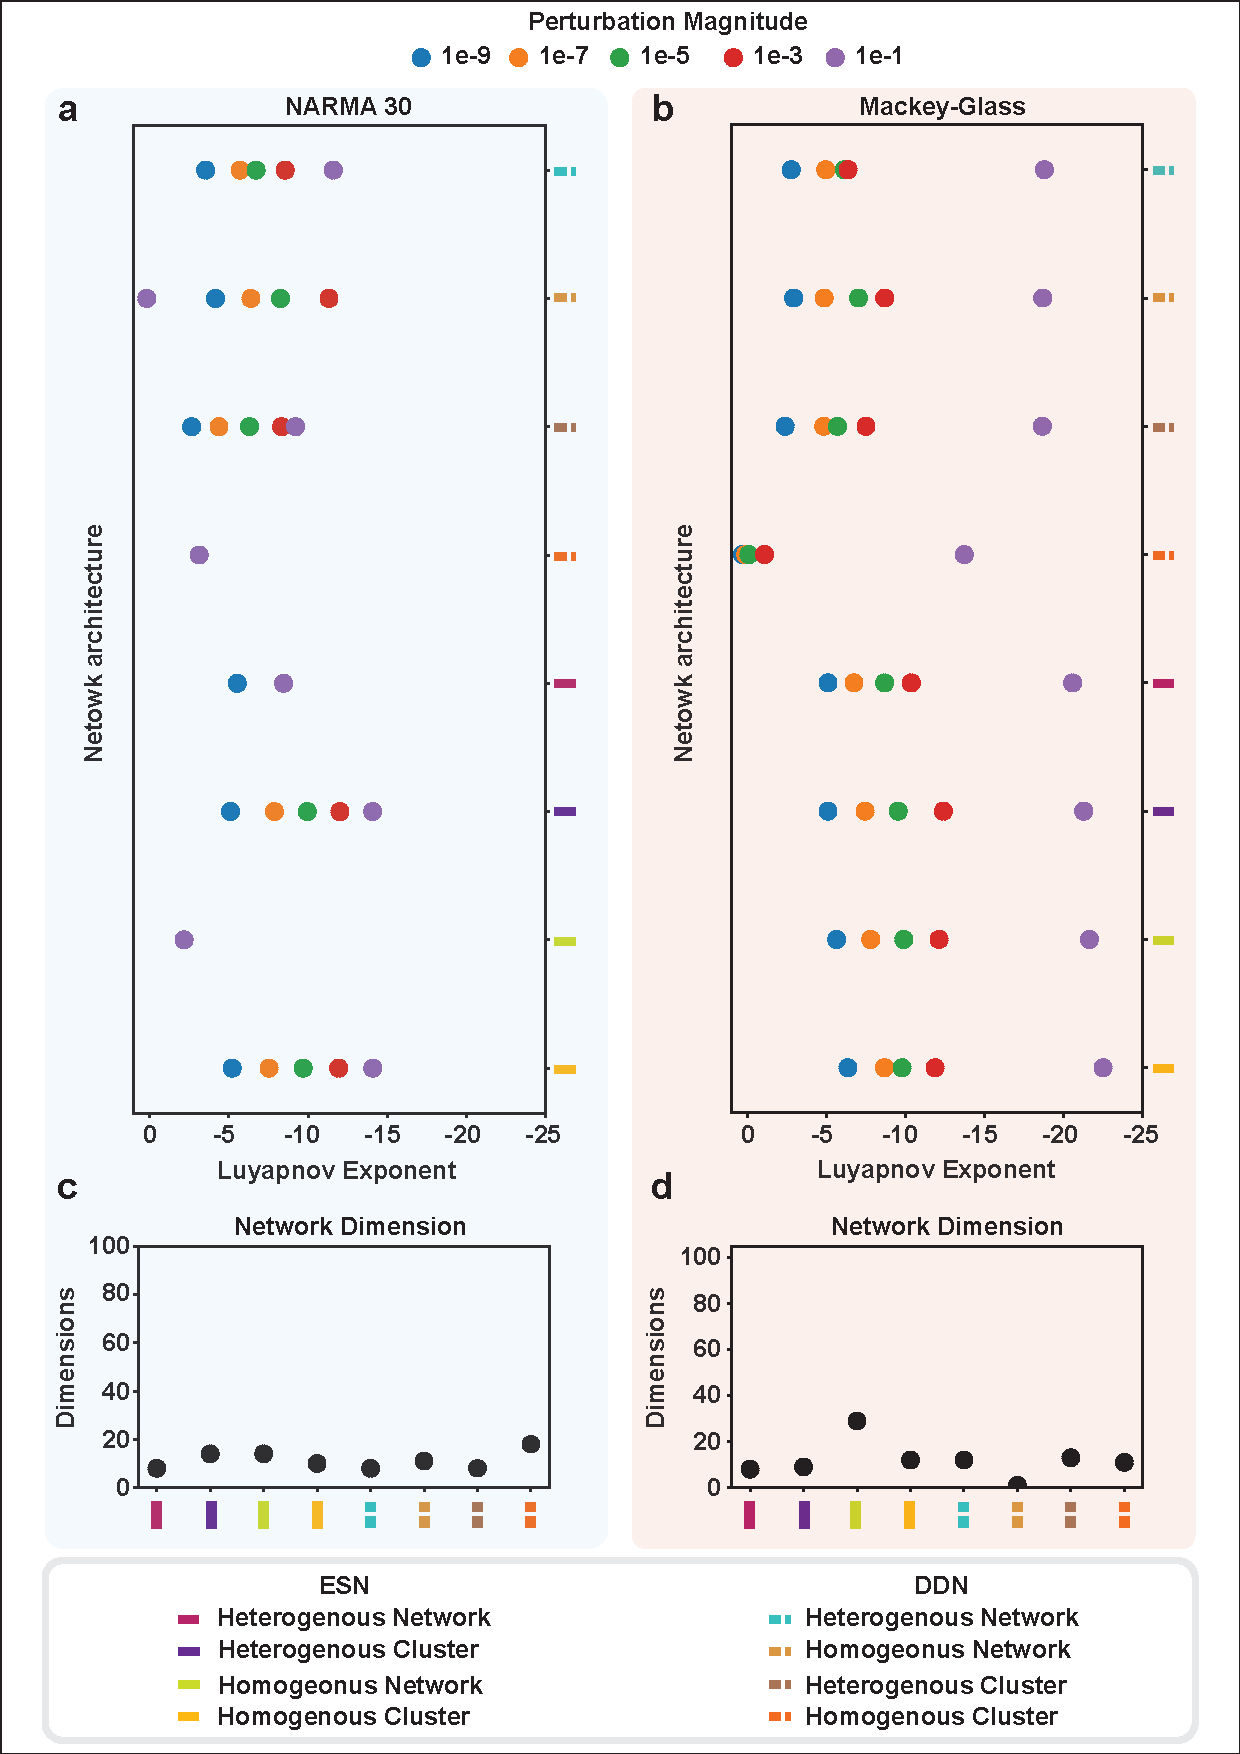
\includegraphics[width=0.8\linewidth]{Figures/Ch_4/Luyapnov_dimensions.pdf}
    \caption{\textbf{Dynamics based on Lyapunov exponent and dimensionality of optimized networks:} \textbf{(a-b)} shows the Lyapunov exponents of the optimized networks while performing the NARMA 30  (blue background) and Mackey-Glass (red background). \textbf{(c-d)} shows the network dimensionality while performing the NARMA 30 (blue background) and Mackey-Glass timeseries prediction tasks (red background).}
    \label{fig:lyapunov}
\end{figure}



\begin{figure}
    \centering
    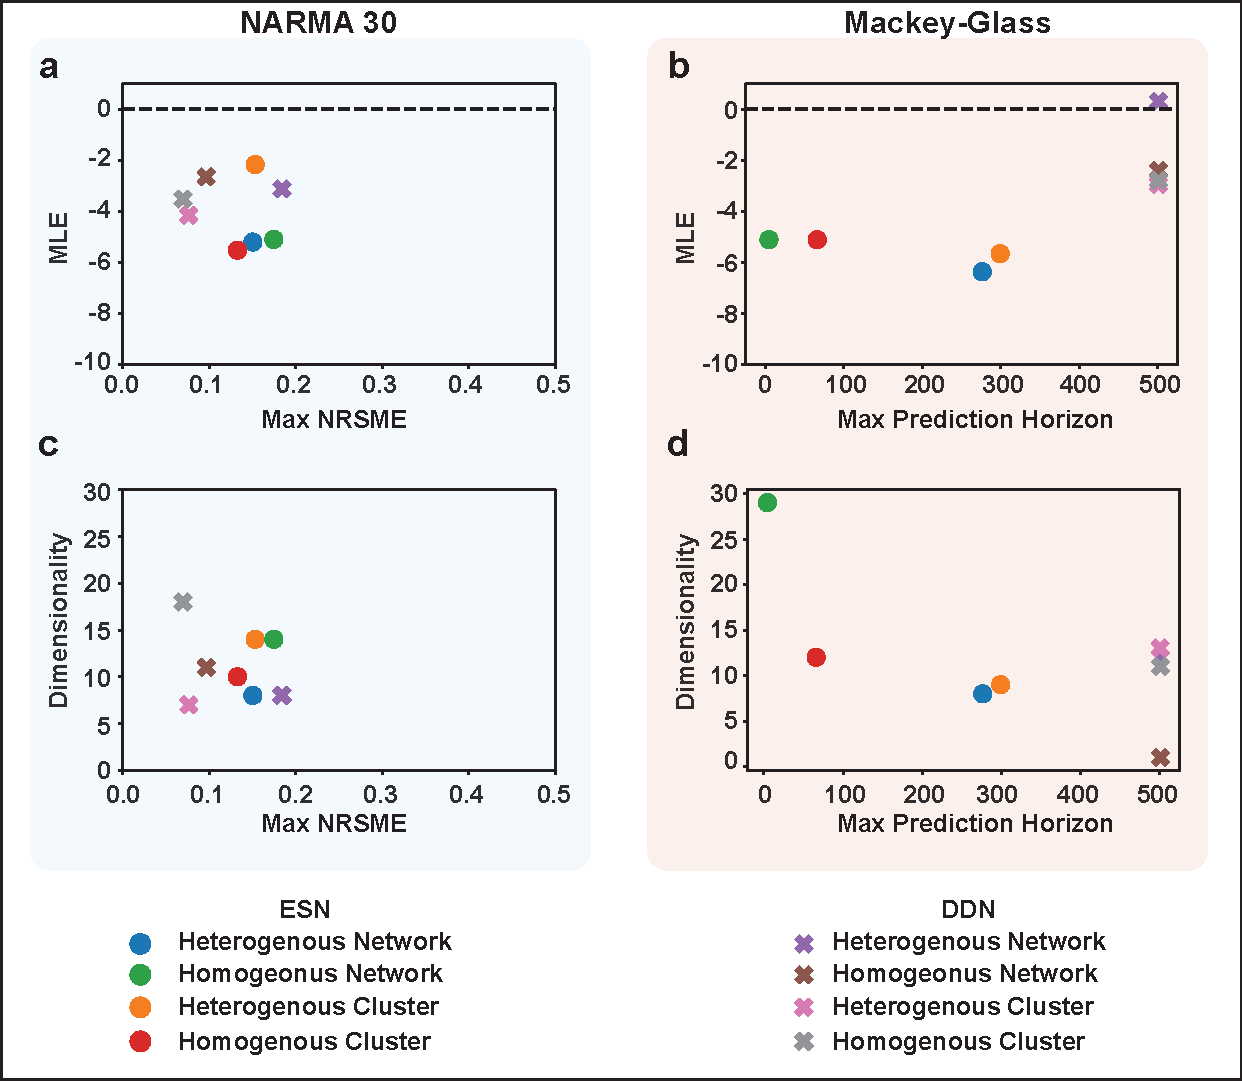
\includegraphics[width=\linewidth]{Figures/Ch_4/LE_DIM_VS_VAL_SCORES.pdf}
    \caption{\textbf{Performance vs stability and Dimensionality} (\textbf{a-b}) shows the maximum LE at the lowest perturbation magnitude (1e-9) vs maximum validation score for the most optimized networks while performing the NARMA 30 (blue background) and Mackey-Glass (red background). \textbf{(c-d)} shows the network dimensionality vs maximum validation score reached while performing the NARMA 30 (blue background) and Mackey-Glass timeseries prediction tasks (red background).}
    \label{fig:lyapunov_vs_perf}
\end{figure}

\subsection{Linear Memory capacity}

Next, we calculated the linear memory capacity (see methods section and \cite{jaeger2001short, jaeger2004harnessing}) to in order to understand if intrinsic decay heterogeneity has an effect on the memory of ESNs and DDNs. This is especially to see if networks with heterogeneous decay parameters change the way networks store temporal information. Specifically, the maximum number of time steps from which these networks can recall information. We used the time window of 40 steps. The observed linear memory capacity for each network variant is summarized in \textbf{Fig. \ref{fig:MC}}. 


For the NARMA-30 task (\textbf{Fig. \ref{fig:MC} left}), it can be seen that every ESN variant has the capacity to recall from up to 20 time steps ago and this capacity is distributed over all the steps between 0 and 20. We do not observe a stark improvement in the memory capacity as a result of heterogeneity.  On the other hand, DDNs show a much more nuanced difference in terms of memory distribution for NARMA-30 task. DDNs with a fixed decay per cluster show a concentration of memory capacity at 3 different time lags, while DDNs with a distributed decay per cluster show a prominent concentration at two lags. It can also be observed that DDNs do not utilize the lags closer to the input (Max Delays = 0), except for DDNs with network wide fixed decay. This suggests that ESNs have a limited capacity to recall the past steps in order to perform the task, and decay heterogeneity doesn't provide any improvement on this. DDNs on the other hand can scatter their capacity more sparsely, therefore utilizing the past states more strategically.         

For the Mackey-Glass time series prediction task (\textbf{Fig. \ref{fig:MC} left}), it can be seen that every ESN variant ustilizes just a few past states from when the input is received, most of the capacity is recruited from just the previous step. We do not observe a stark improvement in the memory capacity as a result of heterogeneity for the case of Mackey-Glass as well. On the other hand, DDNs show a much more variability: DDNs with network wide distributed decay and DDNs with distributed decay per cluster, show a wide spread of memory capacity over multiple delay steps, while DDNs with fixed values show a concentration of capacity around 10 time steps ago. 

In conclusion, while for ESNs the decay heterogeneity doesn't change drastically with memory capacity, for DDNs, the memory capacity is altered by decay heterogeneity. 

\begin{figure}
    \centering
    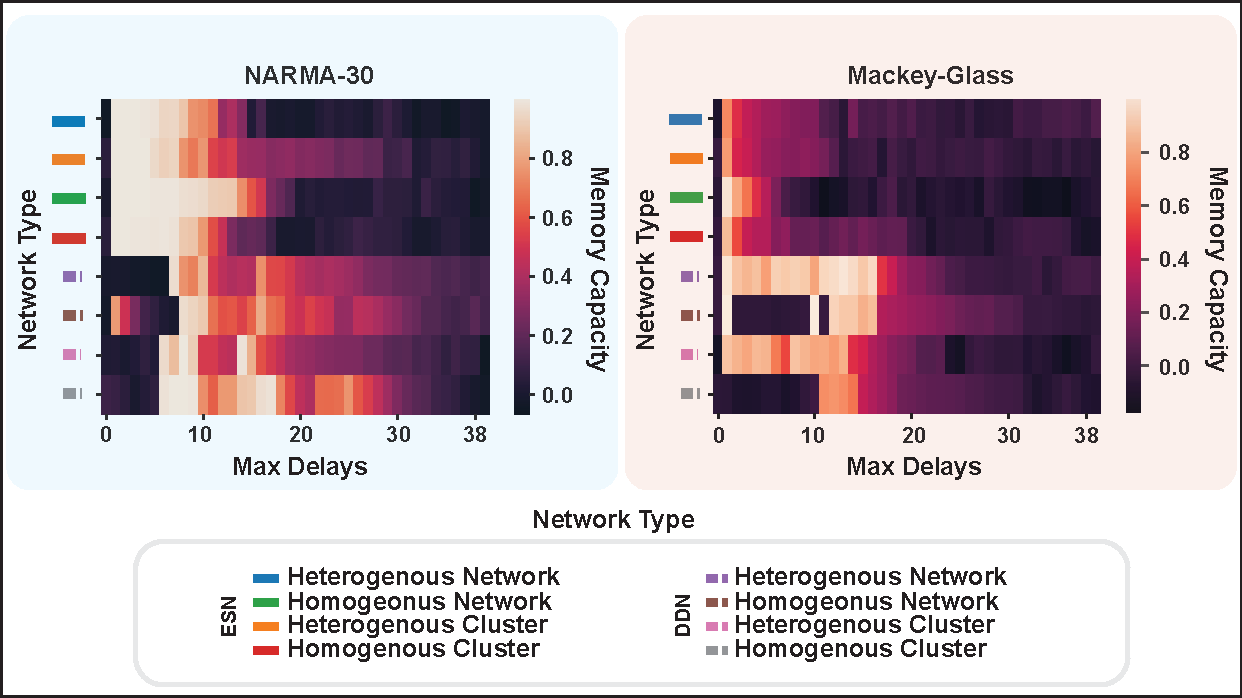
\includegraphics[width=\linewidth]{Figures/Ch_4/LInear MC.pdf}
    \caption{\textbf{Linear Memory Capacity of optimized networks}: \textbf{(Left)} Linear memory capacity of the networks optimized for NARMA 30 task for different delays. \textbf{(Right)} Linear memory capacity of the networks optimized for Mackey-Glass time series prediction task for different delays. }
    \label{fig:MC}
\end{figure}




\newpage


\section{Discussion}


This study aimed at analyzing the effect of timescale (decay parameter) heterogeneity of individual units in reservoir networks on their computational performance, particularly in ESNs and DDNs. Set across two benchmark tasks namely, NARMA-30 and Mackey-Glass, and across four heterogeneity configurations. We found that across all heterogeneity configurations, DDNs outperform ESNs in both tasks. This is in agreement with previous work which showed that delay-based architectures are better suited for memory-intensive tasks (\cite{iacob2022distance}), as the introduction of time delays enables more flexible temporal dynamics. 

We observe that introducing decay time heterogeneity does not increase performance of DDNs further, probably because after a sufficient level, decay heterogeneity becomes redundant. We observed that for ESNs trained on the NARMA-30 task, the homogeneous cluster configuration performs the best. Moreover, for the Mackey-Glass task, ESNs with heterogeneous clusters show the best performance. Surprisingly, homogeneous network DDNs outperform heterogeneous network ESNs, suggesting that architectural delay mechanisms alone offer substantial computational benefits, that extends the hypothesis of (\cite{tanaka2022reservoir}) which claims that diverse timescales enhance network performance in both DDNs and ESNs.

The ultimate best-performing configuration across both tasks were the homogeneous cluster DDNs. This suggests that structured, modular heterogeneity in decay parameters along with delays inherent to DDNs, is more beneficial than randomly distributed heterogeneity. One likely reason is that this setup creates functionally specialized subpopulations with different integration windows, which are quite common in biological neural circuits. Such clusters allows the reservoir to simultaneously retain short and long term dependencies spread across multiple sub reservoirs with distinct decay distribution compared to network wide heterogeneous DDNs where decays are sampled from the same distribution. These results support the hypothesis rooted in neuroscience that the diversity of timescales i.e delay for individual nodes is functionally beneficial for temporal processing and memory (\cite{Lundqvist2016gamma, Runyan2017timescales, Cavanagh2020diverse}). 

Contrary to our initial hypothesis, networks with decay heterogeneity did not show increased instability. In fact, all ESNs remained in a contracting regime, with strongly negative Lyapunov exponents across perturbation magnitudes. DDNs were more variable, with some configurations (e.g., homogeneous network) approaching neutral or even slightly positive exponents under high perturbations. This suggests that DDNs trade off stability for richer dynamics, and that despite heterogeneity in decay parameters, the stability remains intact for low to moderate perturbations. Interestingly, for all network types, the largest perturbation magnitude yielded the most negative Lyapunov exponent. This is likely due to saturation or nonlinear contraction in state space, and highlights the importance of evaluating stability in the local (infinitesimal) regime to interpret true Lyapunov behavior.

We hypothesized that decay heterogeneity would increase the effective dimensionality of the network enabling richer representations. This was not supported by our results. Most networks exhibited relatively low-dimensional dynamics, with little difference between configurations. This could mean that the tasks at hand do not require high-dimensional embeddings, or that the reservoirs learn to compress relevant dynamics efficiently regardless of heterogeneity, this relates to the Neural Task Complexity framework (NTC) (\cite{gao2015simplicity}), which finds low dimensional dynamics in large neural recordings. It may also suggest that stability and memory, not dimensionality, are the primary contributors to performance in this setting.

Linear memory capacity analysis revealed a nuanced story. While ESNs showed limited changes across heterogeneity types, DDNs exhibited significant differences among the heterogeneity configurations in how memory gets distributed. Notably, DDNs with distributed decay showed a wider memory spread, while fixed-decay variants concentrated memory at specific lags. This suggests that decay heterogeneity allows DDNs to strategically allocate memory, a critical property for tasks like NARMA, where both recent and delayed inputs matter. This behavior was absent in ESNs, which tended to have more rigid, shallow memory profiles regardless of heterogeneity.

This study is limited to two benchmark tasks and a specific class of recurrent models. Future work should explore: Broader tasks, including those involving categorical sequence prediction or noisy real-world data, other forms of heterogeneity (e.g., in connectivity, input weights), how decay heterogeneity interacts with delay heterogeneity under more complex learning rules or online adaptation. It would also be valuable to explore the Information processing capacity of these systems, and how dimensionality evolves over time or under different input statistics.



This work focused on two classical benchmarks and a single reservoir framework, but its broader implications invite several extensions. For example, (\cite{gast2024neural}) demonstrate that threshold heterogeneity for excitatory neurons in spiking neural networks  improves encoding task by increasing the dimensionality; building on their insights, future studies might examine how intrinsic decay heterogeneity interacts with learned delay adaptations under continual learning protocols. It will also be important to validate these findings on richer problem domains. For instance, categorical sequence classification and forecasting in real-world, noisy data streams to assess whether heterogeneous timescales confer the same benefits when synaptic inputs are irregular or structured by sensory statistics. Moreover, exploring additional heterogeneity facets, such as variable input-weight distributions or connectivity motifs, could reveal complementary routes to multi-timescale computation. Finally, applying information-processing–capacity analyses to track how representational dimensionality and memory resources reconfigure over learning will clarify the dynamic interplay between architectural heterogeneity and the evolving requirements of complex tasks. 

Our results suggest that introducing modular heterogeneity in decay dynamics can meaningfully improve performance and memory organization in reservoir networks particularly when paired with architectural delays. From a neuroscience perspective, this supports the idea that diverse time constants in biological systems are not arbitrary, but serve computational roles such as memory stratification and temporal coding.

From an engineering viewpoint, these findings argue for designing non-uniform, structured reservoirs in artificial systems, especially for tasks involving long-timescale dependencies or multi-timescale dynamics. Rather than tuning a single decay or leak parameter, practitioners could benefit from multi-cluster architectures with targeted decay profiles.



\newpage


\begin{spacing}{1.0} % Set the line spacing to single spacing
\fontsize{8pt}{8pt}\selectfont
\bibliographystyle{apalike} %%%%Changed
\renewcommand{\bibname}{References}
\bibliography{All_bibtex} %%%%Changed
\end{spacing} % restore the line spacing to original
% \printbibliography